%!TEX ROOT=../../_main.tex

Problém proudění či mechanika tekutiny je v rámci této práce chápán jako zkoumání pohybu velkého množství částic a jejich interakce. Velké množství ve smyslu, že zkoumané fluidum má takovou hustotu, že lze použít aproximaci reality pomocí matematického kontinua. To nám říká, že i v nekonečně malá (infinitesimální) část tekutiny obsahuje dostatečný počet částic, pro které lze specifikovat střední rychlost a střední kinetickou energii. Jsme tak schopni definovat pojmy rychlost, tlak, teplota, hustota a další důležité veličiny jako spojité funkce v rámci celého kontinua. Tato kapitola vychází různou měrou z publikací \cite{blazek2015computational, dvorak1987vnitrniaerodynamika, hirsch2007numerical, shapiro1953dynamics, furst2020mko2}

\section{Základy matematického popisu proudění} \label{sec:zaklady_popisu}

Odvození základních rovnic mechaniky tekutin se opírá tzv. zákony zachování. Pro případ obecné tekutiny to jsou
\begin{enumerate}
	\item zachování hmoty
	\item zachování hybnosti a
	\item zachování energie.
\end{enumerate}
Pro případ nestlačitelné tekutiny si pak vystačíme pouze s prvními dvěma zmíněnými zákony zachování.

Zachování určité veličiny znamená, že její časovou změnu uvnitř libovolného objemu lze vyjádřit jako množství veličiny proudící přes hranici zvoleného objemu a produkci veličiny uvnitř objemu. Často se také mluví o bilanci veličiny v určitém objemu. Množství veličiny, které proudí přes hranici objemu se nazývá tok. Obecně se tok dá rozdělit na dvě složky. Konvekci, způsobenou konvektivním přenosem veličiny, a difuzi, způsobenou pohybem molekul tekutiny v klidovém stavu. Difuzivní přenos závisí na gradientu dané veličiny a pro případ homogenní distribuce tedy vymizí.

\subsection{Kontrolní objem a zákon zachování}\label{sec:kontrolni_objem}
V předchozí kapitole se o zákonech zachování mluvilo v kontextu jistého objemu. Takovémuto libovolně zvolitelnému objemu se často říká kontrolní objem, nebo - pro účely numerické matematiky vhodněji - konečný kontrolní objem.

Mějme obecný kontrolní objem $\Omega$ s uzavřenou hranicí $\Gamma$, který je pevný v prostoru s daným proudovým polem jak naznačuje obrázek \ref{fig:kontrolni-objem}. Zároveň lze definovat element hranice $\mathrm{d}S$ a jeho vnější normálu $\mathbf{n}$.
\begin{figure}[h]
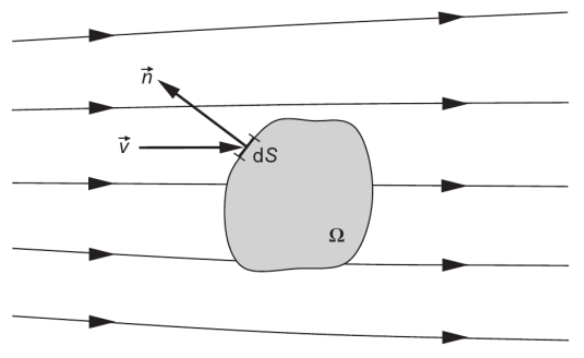
\includegraphics[width=0.7\textwidth]{img/kontrolni_objem.png}
\caption{Pevný kontrolní objem v obecném proudovém poli. \cite{blazek2015computational} PREDELAT PODLE ZNACENI V TEXTU}
\label{fig:kontrolni-objem}
\end{figure}

Pro obecnou zachovávanou veličinu $W$ lze zákon zachování psát jako
\begin{equation}\label{eq:zachovani}
\dfrac{\partial}{\partial t} \int_{\Omega}W\,\mathrm{d}V + \int_{\Gamma}\mathbf{F}(W) \cdot \mathbf{n} \, \mathrm{d}S = \int_{\Omega}Q_\Omega(W) \, \mathrm{d}V + \int_{\Gamma} \mathbf{Q_\Gamma}(W) \cdot \mathbf{n} \, \mathrm{d}S,
\end{equation}
kde $Q_{\Omega}(W)$ jsou objemové a  $\mathbf{Q_\Gamma}(W)$ povrchové zdroje a $\mathbf{F}(W) $ je vektor hustoty toku veličiny $W$ plochou $\Gamma$. Zákon v této formě je formálně platný jak pro skalární veličinu $W$ tak vektorovou $\mathbf{W}$. Speciálně pak pro skalární veličinu lze člen s tokem přes hranici rozdělit, podle dříve zmíněného dělení, na konvektivní tok
\begin{equation}\label{eq:konv_tok}
\mathbf{F_K}(W) = W\mathbf{u}
\end{equation}
a difuzivní tok vyjádřený pomocí zobecněného Fickova gradientního zákona
\begin{equation}\label{eq:diff_tok}
\mathbf{F_D}(W) = \kappa \rho \nabla(W/\rho),
\end{equation}
kde $\kappa$ je koeficient difuzivity a dohromady tedy
\begin{equation*}
\int_{\Gamma}\mathbf{F}(W) \cdot \mathbf{n} \, \mathrm{d}S = \int_{\Gamma}W\left[\mathbf{u}\cdot\mathbf{n}\right] - \kappa \rho \left[\nabla(W/\rho)\cdot \mathbf{n} \right] \mathrm{d}S.
\end{equation*}
Rovnici \ref{eq:zachovani} tak můžeme rozepsat do podoby
\begin{equation}\label{eq:zachovani_skalarStoky}
\dfrac{\partial}{\partial t} \int_{\Omega}W\,\mathrm{d}V + \int_{\Gamma}W\left[\mathbf{u}\cdot\mathbf{n}\right] - \kappa \rho \left[\nabla(W/\rho)\cdot \mathbf{n} \right] \mathrm{d}S = \int_{\Omega}Q_\Omega(W) \, \mathrm{d}V + \int_{\Gamma} \mathbf{Q_\Gamma}(W) \cdot \mathbf{n} \, \mathrm{d}S.
\end{equation}
Pro vektorovou veličinu lze udělat velmi podobné rozdělení, pouze s tím rozdílem, že všechny tři funkce $W$ ($\mathbf{F}, Q_{\Omega}, \mathbf{Q_\Gamma}$) budou o jeden tenzorový řád vyšší. Rovnice \ref{eq:zachovani} s rozdělením na tenzory konvektivního a difuzivního toku tak dostane podobu
\begin{equation}\label{eq:zachovani_vektor}
\dfrac{\partial}{\partial t} \int_{\Omega}\mathbf{W} \, \mathrm{d}V + \int_{\Gamma}\left(\mathbb{F}_K(\mathbf{W})-\mathbb{F}_D(\mathbf{W}) \right)\cdot \mathbf{n} \, \mathrm{d}S = \int_{\Omega} \mathbf{Q_\Omega}(\mathbf{W}) \, \mathrm{d}V + \int_{\Gamma} \mathbb{Q}_\Gamma(\mathbf{W}) \cdot \mathbf{n} \, \mathrm{d}S.
\end{equation}
Takto odvozený obecný zákon zachování (někdy taky bilanční rovnici) lze využít pro odvození základních rovnic proudění.



\subsection{Zákon zachování hmoty, Rovnice kontinuity}
Pro jednosložkové tekutiny vyjadřuje zákon zachování hmoty, tedy že hmotu v systému nelze vytvořit, ani ztratit, i.e. zdroj hmoty se uvnitř kontrolního nepředpokládá. Musí tedy platit, že změna hmotnosti uvnitř kontrolního objemu musí být rovna toku hmoty přes hranice kontrolního objemu, tedy
\begin{equation*}
-\dfrac{\partial}{\partial t}\int_\Omega \rho \,\mathrm{d}V = \int_\Gamma \rho \, u_i \, n_i \mathrm{d}S = \int_\Omega \dfrac{\partial\left(\rho u_i\right)}{\partial x_i}\mathrm{d}V.
\end{equation*}
\nomenclature[P]{$\dfrac{\partial}{\partial w}$}{Parciální derivace podle veličiny $w$}
\nomenclature[D]{$t$}{Čas}
\nomenclature[U]{$u_i,\, \mathbf{u}$}{Vektor rychlosti}
\nomenclature[N]{$n_i,\, \mathbf{n}$}{Normálový vektor hranice}
\nomenclature[R]{$\rho$}{Hustota}
\nomenclature[O]{$\Omega$}{Kontrolní objem}
\nomenclature[G]{$\Gamma$}{Hranice kontrolního objemu}
Po převedení obou integrálů na jednu stranu, záměně operací integrace a derivace a vyžití distributivity integrálu vzhledem k operaci součet, dostáváme obecný tvar rovnice kontinuity pro nestacionární proudění stlačitelné tekutiny
\begin{equation}\label{eq:kontinuita_stlacitelna}
\dfrac{\partial \rho}{\partial t} + \dfrac{\partial \left(\rho u_i\right)}{\partial x_i} = 0.
\end{equation}
Ke stejné rovnici dojdeme, pokud do rovnice zachovaní \ref{eq:zachovani_skalarStoky} dosadíme za obecnou skalární veličinu $W$ hustotu $\rho$, uplatníme předpoklad nulových zdrojů na pravé straně a uvědomíme si, že difuzivní tok z rovnice \ref{eq:diff_tok} bude nulový, neboť 
\begin{equation*}
\nabla(W/\rho) = \nabla(\rho/\rho) = \nabla(1) = 0.
\end{equation*} 
Za předpokladu nestlačitelnosti tekutiny, tedy že $\rho = konst.$ lze navíc rovnici \ref{eq:kontinuita_stlacitelna} zjednodušit na 
\begin{equation}\label{eq:kontinuita_nestlacitelna}
\dfrac{\partial u_i}{\partial x_i} = \nabla\cdot\mathbf{u} = 0,
\end{equation}
což se běžně označuje jako rovnice kontinuity pro proudění nestlačitelné tekutiny (v indexovém a vektorovém zápisu).

\subsection{Zákon zachování hybnosti, Rovnice hybnosti}
Odvození rovnice hybnosti vychází z druhého Newtonova zákona, který říká, že změna hybnosti je způsobena součtem sil účinkujících na element hmotnosti.
Hybnost nekonečně malé části kontrolního objemu je\begin{equation*}
\rho \mathbf{u}\,\mathrm{d}V
\end{equation*}
a tedy změna hybnosti uvnitř kontrolního objemu je
\begin{equation*}
\dfrac{\partial}{\partial t}\int_\Omega\rho\mathbf{u}\,\mathrm{d}V.
\end{equation*}
Sledovanou zachovávanou veličinou vektorovou veličinou $\mathbf{W}$ z analogie předchozího vztahu s prvním členem rovnice \ref{eq:zachovani_vektor} je hybnost $\rho \mathbf{u}$. Formálním použitím rovnice \ref{eq:konv_tok} dostáváme vztah pro tenzor konvektivního toku
\begin{equation*}
\mathbb{F}_K(\mathbf{\rho\mathbf{u}})\cdot \mathbf{n}=\rho\mathbf{u} (\mathbf{u}\cdot\mathbf{n})
\end{equation*}
Difuzivní tok zůstává nulový neboť hybnost nemůže difundovat v tekutině za klidového stavu.

Nejdůležitější částí odvození rovnice hybnosti je interpretace zdrojových členů. Zdroj hybnosti je z hlediska fyziky vždy síla.
\begin{enumerate}
	\item Objemové síly působí na hmotu v celém kontrolním objemu e.g. síla gravitační, inerciální, Coriolisova či elektromagnetická etc. 
	\item Povrchové síly působí přímo na povrchu $\Gamma$ kontrolního objemu. Jedná se o deformační působení vnějších sil. Tenzor napětí, kterým se často toto působení vyjadřuje lze rozdělit na sférickou a deviátorovou složku, které v případě tekutin lze interpretovat jako působení tlaku okolí a smykové a normálové napětí vznikající mezi okolím a kontrolním objemem.
\end{enumerate}

Objemové zdroje lze vyjádřit jednoduše. Pokud příslušnou vnější sílu vztáhneme na jednotku objemu $\rho \mathbf{f_e}$ lze psát
\begin{equation*}
\int_{\Omega} \mathbf{Q_\Omega} \mathrm{d}V = \int_{\Omega} \rho \mathbf{f_e} \,\mathrm{d}V.
\end{equation*}
Povrchové zdroje jsou rozdělené na sférické působení okolního tlaku $p$ a tenzor viskózního napětí $\tau$, tedy
\begin{align*}
\mathbb{Q}_\Gamma &= -p \mathbb{I}+\tau, \\
Q_{\Gamma ij}&= -p \delta_{ij}+\tau_{ij},
\end{align*}
kde $\mathbb{I}$ je jednotkový tensor, případně $\delta_{ij}$ Kronekerovo delta. Pro Newtonskou tekutinu lze tenzor viskózního smykového napětí vyjádřit podle \cite{hirsch2007numerical} jako 
\begin{equation*}
\tau_{ij}=\mu \left[ \left( \dfrac{\partial u_j}{\partial x_i} + \dfrac{\partial u_i}{\partial x_j} \right) - \dfrac{2}{3} \delta_{ij} \left(\nabla \cdot \mathbf{u}\right)  \right],
\end{equation*}
za předpokladu konstantní dynamické viskozity $\mu$ jak poukazuje \cite{dvorak1987vnitrniaerodynamika}.

Nyní lze již psát soustavu pohybových Navier-Stokesových (NS) rovnic v integrálním tvaru, tedy rovnice hybnosti pro stlačitelnou Newtonskou tekutinu, jako
\begin{equation*}
\dfrac{\partial}{\partial t} \int_{\Omega} \rho \mathbf{u} \,\mathrm{d}V + \int_{\Gamma} \rho \mathbf{u} (\mathbf{u}\cdot \mathbf{n}) + p\mathbf{n} - \tau \cdot \mathbf{n} \,\mathrm{d}S = \int_\Omega \mathbf{Q_\Omega} \,\mathrm{d}V.
\end{equation*}

Často lze rovnici hybnosti nalézt i v diferenciálním tvaru, například v \cite{hirsch2007numerical}
\begin{equation*}
\rho \dfrac{\partial \mathbf{u}}{\partial t} + \rho (\mathbf{u} \cdot \nabla)\mathbf{u} +\nabla p - \mu \left[ \Delta \mathbf{u} + \dfrac{1}{3} \nabla(\nabla \cdot \mathbf{u}) \right] = \rho \mathbf{f_e}
\end{equation*}

\subsection{NS rovnice pro nestlačitelnou tekutinu}

Obecný systém NS rovnic lze pro speciální případy zjednodušit zanedbáním některých fyzikálních vlivů. 
V této práci budeme později využívat zjednodušený tvar NS rovnic  pro nestlačitelnou tekutinu. 
Tedy $\rho=konst.$ čímž dostáváme rovnici kontinuity ve zjednodušeném tvaru \ref{eq:kontinuita_nestlacitelna}, tedy
\begin{equation*}
\nabla\cdot\mathbf{u} = 0
\end{equation*}
a NS rovnice hybnosti v diferenciálním tvaru podle \cite{hirsch2007numerical} má podobu 
\begin{equation}\label{eq:NS_icoDiff}
\rho \dfrac{\partial \mathbf{u}}{\partial t}+ \rho(\mathbf{u}\cdot \nabla)\mathbf{u} = -\nabla p + \mu \Delta \mathbf{u} + \rho \mathbf{f_e}.
\end{equation}
Rovnici hybnosti jde dále vydělit konstantou hustoty, čímž dostaneme jakýsi měrný tlak $ \widehat{p} = \dfrac{p}{\rho} $ a rovnice \ref{eq:NS_icoDiff} přejde do tvaru
\begin{equation}\label{eq:NS_icoPseudotlak}
\dfrac{\partial \mathbf{u}}{\partial t}+ (\mathbf{u}\cdot \nabla)\mathbf{u} = -\nabla \widehat{p} + \mu \Delta \mathbf{u} + \mathbf{f_e}.
\end{equation}



\section{Základ metody konečných objemů}
Metoda konečných objemů (MKO, anglicky Finite volume method - FVM) je jednou z nejpoužívanějších metod pro řešení PDR proudění - společně s konečnými diferencemi a metodou konečných prvků. 
Popularita MKO pro numerické řešení problému proudění tkví podle \cite{hirsch2007numerical} v její obecnosti, srozumitelnosti základních principů a snadnosti implementace pro libovolné sítě i složitější geometrie.

Zásadní výhodou z hlediska přesnosti MKO je pak princip tzv. konzervativní diskretizace (konzervativní ve smyslu zachovávající). Udržet v platnosti základní zákony zachování je důležitý aspekt správnosti řešení. MKO má tu výhodu, že konzervativní diskretizace je podle \cite{hirsch2007numerical} splněna automaticky díky přímé diskretizaci integrálního tvaru zákonů zachování. 

\subsection{Konečný objem}
MKO nese svůj název podle způsobu prostorové diskretizace, tj. rozdělení zkoumané oblasti $\Omega=\mathbb{R}^d$ na vzájemně disjunktní neprázdné otevřené podoblasti $\Omega_j$ s konečnou velikostí, matematicky psáno
\begin{align*}
\overline{\Omega} = \cup^n_{i=1}\overline{\Omega}_i,&\\
\Omega_i \cap \Omega_j = \emptyset,& \,\,\mathrm{pro} \, i \neq j.
\end{align*}
Tyto konečné objemy (někdy buňky) jsou analogií kontrolních objemů z podsekce \ref{sec:kontrolni_objem}. Jakmile máme takto rozdělenou výpočetní oblast, tak na každý konečný objem aplikujeme zákon zachování v integrálním tvaru. To si můžeme dovolit, neboť zákony zachování byly v sekci \ref{sec:zaklady_popisu} odvozeny pro libovolný kontrolní objem a lze je tedy aplikovat na každý konečný podobjem zvlášť. Obecný zákon zachování popsaný rovnicí \ref{eq:zachovani} má pro j-tý kontrolní objem tvar
\begin{equation}\label{eq:zachovani_MKO}
\frac{\partial}{\partial t} \int_{\Omega_j}W\,\mathrm{d}V + \int_{\Gamma_j} \mathbf{F} \cdot \mathbf{n} \,\mathrm{d}S = \int_{\Omega_j}Q_\Omega \,\mathrm{d}V,
\end{equation}
kde pro jednoduchost zápisu ponecháváme jen objemové zdroje na pravé straně.
Pro každý konečný objem nyní definujeme prostorově střední hodnotu sledované veličiny 
\begin{equation*}
\overline{W}|_{\Omega_j}= W_j(t) = \frac{1}{|\Omega_j|}\int_{\Omega_j}W(\mathbf{x},t) \,\mathrm{d} V.
\end{equation*}
Stejným způsobem nahradíme i objemové zdroje v rovnici \ref{eq:zachovani_MKO} a integrál toku $\mathbf{F}$ nahradíme součtem přes hranice. Dostaneme tvar rovnice zachování, napsanou pro j-tý kontrolní konečný objem
\begin{equation}\label{eq:polodiskretniMKO}
\frac{\partial}{\partial t} (W_j|\Omega_j|) + \sum_{\forall f} \int_{f}\mathbf{F}\cdot \mathbf{n} \,\mathrm{d}S = Q_j|\Omega_j|,
\end{equation} 
kde stěny $f$ jsou jednotlivé části hranice $\Gamma_j$ a všechny stěny tvoří vzájemně disjunktní pokrytí příslušné hranice.
Stojí za to podotknout, že rovnice \ref{eq:polodiskretniMKO} je stále matematicky ekvivalentní k rovnici \ref{eq:zachovani_MKO}.
Prozatím jsme ještě neprovedly žádné aproximace či přibližné náhrady.

\subsection{Aproximace numerickým tokem}

Nyní se pokusíme aproximovat integrál toku přes hranice z rovnice \ref{eq:polodiskretniMKO}. Pro lepší představu teď předpokládejme, že tok zachovávané veličiny je dán z rovnic \ref{eq:diff_tok} a \ref{eq:konv_tok} jako
\begin{equation*}
\mathbf{F}=\mathbf{u}W-\kappa \nabla W.
\end{equation*}
Tok přes stěnu $f$ (část hranice $\Gamma_j$) se souřadnicí středu $\mathbf{x_f}$ můžeme aproximovat pomocí
\begin{equation}\label{eq:aprox_tok}
\int_{f}\mathbf{F}\cdot \mathbf{n} \,\mathrm{d}S=\int_{f}(\mathbf{u}W-\kappa\nabla W)\cdot \mathbf{n}\, \mathrm{d}S \approx \left(\mathbf{u} W_f - \kappa \nabla W_f \right) \cdot \mathbf{S_f} = \mathbf{F_f} \cdot \mathbf{S_f},
\end{equation}
kde $\mathbf{S_f}=\int_{\Gamma_j}\mathbf{n}\,\mathrm{d}S$, což je konstantní vlastnost geometrie stěny, $W_f(t) = W(\mathbf{x_f},t)$ a $\nabla W_f(t) = \nabla W (\mathbf{x_f}, t)$.

Pro řešení úlohy je také potřeba zvolit, kde budou ukládány proměnné. Jinými slovy, jestli v našich rovnicích bude neznámá např. $W_j$, nebo $W_f$. V praxi se používá více možností i případných kombinací, jak uvádí \cite{blazek2015computational, hirsch2007numerical}.
Standardně se používá ukládání hodnot ve středu buněk, ve středu stěn či ve vrcholech.
V některých případech se objevuje i smíšený způsob (anglicky \textit{staggered}), kde hodnoty různých veličin jsou ukládány na jiných místech.
Dále budeme předpokládat, že proměnné uchováváme ve středu buněk (anglicky \textit{cell-centered}), tedy že proměnnou bude hodnota $W_j$.
Pro další postup je tedy potřeba aproximovat hodnoty $W_f$ a $\nabla W_f \cdot \mathbf{S_f}$ pomocí zavedených neznámých ve středech buněk a získat tak $ \mathbf{F_f} = \mathbf{F_f}(W_j)$.
Poté již můžeme napsat semidiskrétní tvar (ve smyslu MKO) rovnice zachování skalární veličiny 
\begin{equation*}
\frac{\partial}{\partial t} (W_j|\Omega_j|) + \sum_{\forall f} \mathbf{F_f} \cdot \mathbf{S_f} = Q_j|\Omega_j|.
\end{equation*}
Způsobů diskretizace numerického toku je mnoho, neboť jde o jednu ze stěžejních částí MKO. Numerický tok totiž zásadním způsobem ovlivňuje stabilitu a přesnost následného výpočtu. Dále jsou uvedeny pouze základní příklady způsobu diskretizace, neboť jejich rozbor není předmětem této práce.

\subsubsection{Diskretizace difuzivního toku}
Jak uvádí rovnice \ref{eq:aprox_tok}, aproximujeme člen difuzivního toku přes stěnu $f$ jako
\begin{equation*}
-\int_f \kappa \nabla W \mathrm{d}S \approx \mathbf{F_D} = -\kappa \nabla W_f \cdot \mathbf{S_f}.
\end{equation*}
Pro diskretizaci takového členu můžeme vztah upravit na
\begin{equation*}
\mathbf{F_D} = -\kappa \dfrac{\partial W_f}{\partial \mathbf{n_f}} S_f,
\end{equation*}
kde $\dfrac{\partial W_f}{\partial \mathbf{n_f}}$ je tzv. derivace ve směru normály stěny $f$ a $S_f$ je plocha stěny. Pokud stěna $f$ je právě mezi buňkami $ j=C $ a $ j=N $, tak lze derivaci ve směru aproximovat pomocí 
\begin{equation*}
\dfrac{\partial W_f}{\partial \mathbf{n_f}} \approx \dfrac{W_N-W_C}{||\mathbf{x_N}-\mathbf{x_C}||}.
\end{equation*}

\subsubsection{Diskretizace konvektivního toku}


\section{SIMPLE algoritmus}
myslenka, 'podvod', relaxace

\section{Turbulence, modelování turbulence}
v rychlosti o RANS, model turbulence Spalart a K-Omega rozdil vyhody a vhodnost aplikace (ucel modelu)